\section{Modules Analysis}
\label{sec:modules_analysis}

This section examines each of the four functional modules of the current system in detail: data ingestion, data storage, data visualisation, and recommendation.

\subsection{Data Ingestion Module}
\label{sec:ingestion_analysis}

The data ingestion module is responsible for loading raw item and interaction data into the system's storage layer.
In the current implementation, ingestion is performed as an offline batch process.
A set of pre-processing scripts reads source files (Amazon Book Reviews JSON dumps and item metadata CSVs), parses records, applies minimal schema validation (checking for required fields), and bulk-inserts the resulting documents into MongoDB.
Figure~\ref{fig:ingestion_pipeline} illustrates the ingestion pipeline.

\begin{figure}[H]
\centering
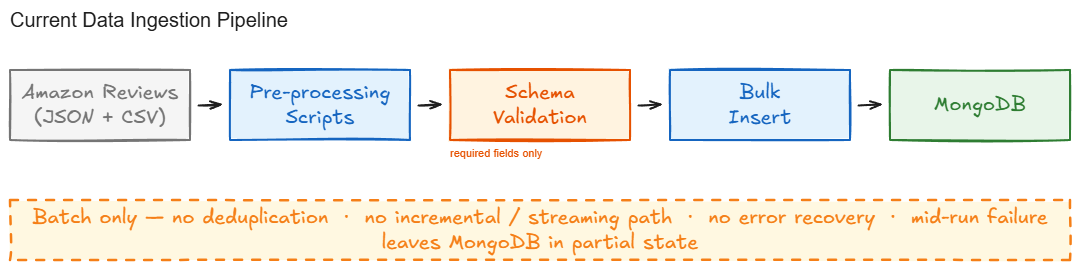
\includegraphics[width=0.90\textwidth]{images/chapter3/fig_ingestion_pipeline}
\caption{Current data ingestion pipeline. All ingestion is performed offline in batch; there is no streaming or incremental update path.}
\label{fig:ingestion_pipeline}
\end{figure}

Several limitations are evident.
First, the pipeline has no deduplication step: re-running ingestion on an overlapping data slice creates duplicate interaction records in MongoDB, corrupting downstream model training.
Second, schema validation is shallow — only the presence of required keys is checked, without type coercion or range validation, allowing malformed records to pass silently.
Third, the batch-only design means that new data sources (e.g., a live user interaction stream) cannot be incorporated without a full re-run of the entire ingestion pipeline, which takes several hours for the full Amazon dataset.
Fourth, no error recovery mechanism exists: a failure mid-run leaves MongoDB in a partially ingested state that requires manual cleanup.

\subsection{Data Storage Module}
\label{sec:storage_analysis}

The data storage module encompasses MongoDB, Redis, the FAISS index, and the Tantivy index.

\paragraph{MongoDB —}
The application writes to two collections in the \texttt{nba\_logs} database.
The \texttt{interactions} collection receives raw event documents (user ID, item ASIN, action type, timestamp, session ID) via \texttt{insert\_one} as the Redis queue worker drains each entry.
The \texttt{profiles} collection stores the latest aggregated profile for each user and is updated via \texttt{update\_one} with \texttt{upsert=True}.
No indexes are defined programmatically in the application code: neither collection has an explicit index on any field, meaning that profile lookups by \texttt{user\_id} and interaction history scans both require full collection scans as the data grows.

\paragraph{Redis —}
Redis serves as an asynchronous interaction write-queue rather than a cache.
When a user performs an action (click, cart, or skip), the \texttt{/interact} route serialises the event as a JSON document and appends it to the \texttt{nba\_interactions} list via \texttt{RPUSH}, returning immediately to the caller without waiting for a MongoDB write.
A background coroutine started at application startup drains the list using \texttt{BLPOP} with a 5-second timeout, writing each drained entry to MongoDB via \texttt{db.log\_interaction()}.
When the number of drained entries since the last refit reaches a configurable threshold, the worker initiates an asynchronous Cleora graph refit to refresh the behavioural embeddings with the accumulated interaction data.
This decoupling ensures that the high-frequency interaction write path is not blocked by slower MongoDB write latency.

\paragraph{FAISS flat index —}
The current FAISS index is a flat (exact) inner-product index over all 3{,}080{,}829 item embeddings generated by the BLaIR encoder.
Table~\ref{tab:prior_faiss_latency} summarises the measured search latency characteristics.

\begin{table}[H]
\centering
\caption{FAISS flat index search latency in the current system (single-query, CPU).}
\label{tab:prior_faiss_latency}
\begin{tabular}{lr}
\hline
\textbf{Metric} & \textbf{Value} \\
\hline
P50 latency & 612.19 ms \\
P95 latency & 655.22 ms \\
Recall@$k$ & 1.000 (exact) \\
Index size on disk & $\sim$12 GB \\
Load time at startup & $\sim$45 s \\
\hline
\end{tabular}
\end{table}

A P50 latency of 612 ms makes real-time interactive search infeasible; a user issuing a search query must wait over half a second for a response before the BM25 re-ranking stage is even reached.
The index also resides entirely in CPU RAM, which consumes a large portion of available system memory and leaves insufficient headroom for GPU-accelerated encoding.

\paragraph{Tantivy BM25 index —}
The Tantivy index covers item titles and author fields and is served as a read-only index built offline.
Its query performance is satisfactory (sub-10 ms for most queries), but it is not updated incrementally — adding new items requires a full index rebuild.

\subsection{Data Visualisation Module}
\label{sec:viz_analysis}

The data visualisation module is the React frontend described in Section~\ref{sec:overall_arch}.

The current frontend exhibits three principal limitations.
First, the search view renders all results synchronously on the main thread: if the API response is slow (as is common given the flat FAISS latency), the entire page is unresponsive during the request.
Second, there are no filtering or sorting controls — the user cannot restrict results by genre, publication year, or relevance score, and must scroll through the full returned list.
Third, the visualisation layer has no support for multilingual input: the search bar provides no language indicator, no transliteration support, and no feedback when a Vietnamese query yields poor results due to encoder limitations.
The recommendation panel displays a static list that is refreshed only on full page reload, with no indication of which pipeline generated each recommendation.

\subsection{Recommendation Module}
\label{sec:rec_analysis}

The recommendation module in the current system is GRU-SeqDQN, a hybrid sequential-reinforcement learning approach.

A \texttt{DualStreamItemEncoder} projects each item's text embedding (1{,}024-dim, BLaIR) and CLIP image embedding (512-dim) independently into a 512-dimensional space and concatenates them, producing a 1{,}024-dimensional item representation per sequence step.
A three-layer GRU (\texttt{GRU\_HIDDEN\_DIM} = 512) processes the packed sequence of item representations and produces a fixed-length user state $\mathbf{h}_T \in \mathbb{R}^{512}$.
The \texttt{SequentialDQN} scorer concatenates $\mathbf{h}_T$ with the candidate item representation (512 + 1{,}024 = 1{,}536 dimensions) and passes it through three fully connected layers (1{,}024 → 512 → 256 → 1) to output a scalar Q-value for that candidate.

Training is performed online via experience replay: every click and cart event triggers a \texttt{train\_step} call that pushes the transition $(s_t, a_t, r_t, s_{t+1})$ to a replay buffer and immediately samples a mini-batch to update the network by minimising the Bellman error.

Two structural weaknesses are observable from the design.
First, the GRU hidden state is a fixed-size bottleneck: for users with hundreds of interactions, the model must compress a long, diverse sequence into a 512-dimensional vector using a truncated window of only \texttt{MAX\_SEQ\_LEN} = 50 steps, discarding any context from earlier in the history.
Second, the DQN action space is the full 3-million-item catalogue, which is far too large for Q-value estimation to converge reliably; the effective action space seen during online training is limited to items that happen to appear in user sessions, creating severe distributional shift for long-tail items.
These weaknesses are confirmed quantitatively in Chapter~5, where GRU-SeqDQN achieves HR@10 = 0.0823 — near the random baseline of 0.1000.

